%% Template for MLP Coursework 4

%% Based on  LaTeX template for ICML 2017 - example_paper.tex at 
%%  https://2017.icml.cc/Conferences/2017/StyleAuthorInstructions


\documentclass{article}
\usepackage[T1]{fontenc}
\usepackage{amssymb,amsmath}
\usepackage{txfonts}
\usepackage{microtype}
\usepackage{xspace}
\xspaceaddexceptions{\%}

% Lists with less spacoing between items
\usepackage{paralist}

% For figures
\usepackage{graphicx}
\usepackage{subfig} 

% For citations
\usepackage{natbib}

% For algorithms
\usepackage{algorithm}
\usepackage{algorithmic}

% the hyperref package is used to produce hyperlinks in the
% resulting PDF.  If this breaks your system, please commend out the
% following usepackage line and replace \usepackage{mlp2017} with
% \usepackage[nohyperref]{mlp2017} below.
\usepackage[hyphens]{url}
\urlstyle{same}
\usepackage{hyperref}

% Packages hyperref and algorithmic misbehave sometimes.  We can fix
% this with the following command.
\newcommand{\theHalgorithm}{\arabic{algorithm}}


% Set up MLP coursework style (based on ICML style)
\usepackage{mlp2019}
\mlptitlerunning{MLP Coursework 3 -- Interim Report (\groupNumber)}
\bibliographystyle{icml2017}


\DeclareMathOperator{\softmax}{softmax}
\DeclareMathOperator{\sigmoid}{sigmoid}
\DeclareMathOperator{\sgn}{sgn}
\DeclareMathOperator{\relu}{relu}
\DeclareMathOperator{\lrelu}{lrelu}
\DeclareMathOperator{\elu}{elu}
\DeclareMathOperator{\selu}{selu}
\DeclareMathOperator{\maxout}{maxout}







\usepackage{minted}
\newminted{python}{frame=lines,framerule=2pt}

\usepackage{tikz}
\def\checkmark{\tikz\fill[scale=0.4](0,.35) -- (.25,0) -- (1,.7) -- (.25,.15) -- cycle;} 

% \usepackage{natbib}     %
% \usepackage{natbibspacing}
% \def\BibTeX{{\rm B\kern-.05em{\sc i\kern-.025em b}\kern-.08em
%     T\kern-.1667em\lower.7ex\hbox{E}\kern-.125emX}}




%% You probably do not need to change anything above this comment

%% REPLACE this with your project title, group ID and list of student numbers for the group
\def\projectTitle{Advanced Vision Mini Project}
\def\groupNumber{G007}
\def\studentNumbers{s2196789, s2163307, s2262548, s2203462}

\begin{document} 

\twocolumn[
\mlptitle{\projectTitle: Final Report}
\centerline{\groupNumber\ (\studentNumbers)}

\vskip 7mm
]

\begin{abstract} 
In a deep learning context, training models with limited data remains an open challenge in recent years. In many domains, researchers take the subset of the original dataset to simulate a limited-data environment. In this project, to investigate data efficiency, we trained ResNet-50 on a sub-sampled version of ImageNet-1k with 50 images for each class. As an outcome, our model achieves 20.0\% test accuracy on the VIPriors image classification dataset.

\end{abstract} 

\section{Introduction}
\label{sec:intro}
Lots of computer vision algorithms have been deployed to real-world applications and started to improve our life quality. However, big data and labels are not always available. Sometimes we only have extremely limited labelled data, such as medical images which require experts to label them\cite{yao2021machine}. Under such circumstances of only limited data given, we have successfully implemented an effective image classification task based on Resnet50. Important approaches we adopt to improve the performance of the network include applying frozen models and dropout methods. As regards limited data, multiple data augmentation procedures are carried out to increase the amount of data and reduce overfitting phenomena.  

In the following, we first briefly introduce the limited dataset of the challenge in Section 2 and then provide all technical details of our data preprocessing, adjustment, and training in Section 3. The details and results of our experiments, including experiment environment, settings of hyper-parameters, further modification of our model etc. are presented in Section 4. 


\section{Data set and task} 
\label{sec:task}
\subsection{Data set: ImageNet subset}
ImageNet \cite{deng2009imagenet} is an image dataset organized according to the WordNet \cite{Miller1995} hierarchy. For each concept in the dataset, there are hundreds and thousands of images used for depicting the image class (e.g., daily objects, animals, natural scenes). The dataset holds more than 1M images for training and 50,000 images for validation and 100,000 images for testing, organised in 1,000 categories. In this project, a subset \cite{kayhan2020translation} of the ImageNet dataset was provided for training and validation, which contains only 50 images per class and 50000 images in total. The original validation set was taken to evaluate the models we develop and thus serves as the test set for the project. Therefore, the sizes of the training plus validation set and the test set are both 50,000. 

Because of the limitation of computational resources and drive space, our model would be trained on the reduced data set with all the images resized to $224 \times 224$ pixels. 

\subsection{Task: outperform the baseline resnet50 with limited data}
Since the training data shrinks from 1M to 50,000 images with only 50 images for each class, the training process would be more challenging because such limited data would easily result in an overfitting problem. In this project, the task is performing classification on the subset of ImageNet with ResNet50 \cite{he2016deep}, aiming to achieve higher top-1 classification accuracy based on limited data with deep learning approaches and data augmentation techniques.

\section{Methodology}
\label{sec:methodology}
In this section, our approaches for tackling the challenges of limited data and overfitting will be elaborated, including modifications to the pre-trained baseline model structure and data augmentation strategies adopted during training and inference times. 

\subsection{Baseline model modification}
According to the description in Vipriors challenges \footnote{https://github.com/VIPriors/vipriors-challenges-toolkit/tree/master/image-classification}, the baseline model (Resnet-50 Full-Conv) should achieve 31.16\% accuracy on the test data. However, preliminary experiment observations show that the test accuracy decreased rapidly if the baseline model was trained on the limited dataset with the weights unfrozen. We also observed that the pre-trained Resnet-50 model capable of reaching 26\% accuracy on the test set can only reach about 2-3\% of accuracy on the training set. Based on these abnormal observations, we suspect that the distribution of the limited training data given is inconsistent with that of the data used for training the baseline model since the achieved training accuracy is much lower than the test accuracy. Another speculation is that the baseline model might be suffering from the overfitting problem since its test accuracy drops dramatically as it fits closer to the training data. 

\subsubsection{Freeze model weights}
Since the limited training data given to us in this project as the target domain is a significantly reduced subset of the original ImageNet dataset and we assume that the baseline ResNet-50 model is trained on a different subset of the ImageNet dataset as the source domain, we decide that it is suitable to further leverage the pre-trained weights in the baseline model and employ transfer learning method to address the problem of limited target training data available while the source and target domains have some similarities but are not identical \cite{hussain2018study}. To maintain the pre-trained weights of the baseline model, The last fully-connected layer of the baseline ResNet-50 was removed, and the weights of the remaining layers were frozen as a \textbf{feature extractor} during training.  

\subsubsection{Insert Dropout layer}
Since the baseline model was trained from scratch for 90 epochs on limited data with its test performance severely degraded during training, we suspect that the model might be suffering from overfitting. To mitigate the overfitting problem, we inserted a Dropout layer\cite{srivastava2014dropout} between the feature extractor and the final \textbf{classifier} which is a fully connected layer with 2048 input units and 1000 output units followed by a softmax output layer.
The Dropout layer mitigates overfitting through reducing the dependence between the feature extractor output and the classifier output and achieves such goal by randomly setting the output of feature extractor to zero according to the dropout probability $p$ which is set to be 0.2 in our model. The forward propagation of the Dropout layer during training is defined as following:

\begin{align}
    mask &\sim bernoulli(1-p)\\
    y' &= mask \odot y\
\end{align}

where $y$ is the feature extractor output of shape [1, 2048] after average pooling is applied to the 2048 feature maps in the final convolution layer and $y'$ is the feature extractor output after Dropout is applied. $mask$ is a masking vector also of shape [1, 2048] randomly sampled from the bernoulli distribution with success probability of $1-p$
and $\odot$ denotes the element-wise multiplication.
At inference time however, the classifier output should deterministically depend on the feature extractor output with no stochasticity. And the feature extractor output is scaled down by the inclusion rate $1-p$ to account for the change in its expectation.

\begin{align}
    y' &= y*(1-p)\
\end{align}

And by randomly dropping some of the feature extractor outputs during training, the Dropout layer utilizes a subset of the whole model architecture by averaging the output of different sub networks.
Further, in order to stabilize the input into the classifier and prevent the activation functions from entering saturation zones where the gradients may vanish and to ensure a smoother optimization landscape for the parameters and faster convergence during training \cite{santurkar2018does}, a Batch normalization layer \cite{ioffe2015batch} is added before the Dropout layer to normalize the output of the feature extractor across batches during training. With modifications of the model mentioned above, only the final classifier will be trained in the experiment. 


\subsection{Data augmentation}
The following steps of data augmentation are illustrated using the second image in the resized test dataset named ILSVRC2012\_val\_00000002, as shown below as Figure \ref{fig1}.

%图片处理原图(考虑是否保留)
\begin{figure}[htbp]
\centerline{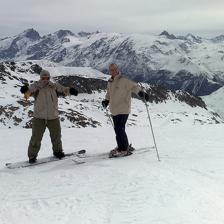
\includegraphics[scale=0.6]{ILSVRC2012_val_00000002.JPEG}}
\caption{The Original ILSVRC2012\textunderscore val \textunderscore00000002}
\label{fig1}
\end{figure}
 

\subsubsection{Random Resized Crop}
The first step is to resize the original photograph and randomly crop it. This comprises two steps, i.e. We firstly resize the graphs and then randomly crop them.

\paragraph{Resizing:}
Resizing is completed by adjusting the shorter edge of the image (symbolized as a vector of $(Width,Hight)$) to the designated pixel value, thus proportionally resizing the entire image, which is simplified as: 
\begin{equation}
f_{resize}((Width,Height))=\begin{cases}
(Width\times \frac{l_r}{Height},l_r), Height\leqslant Width\\
(l_r,Height\times \frac{l_r}{Width}), Height>Width
\end{cases}
\end{equation}
 
Taking ILSVRC2012\textunderscore val \textunderscore00000002 as an example, setting pixels of its shorter edge as 256, we get the image itself before and after being resized shown as Figure \ref{fig2}.

\begin{figure}[htbp]
\centerline{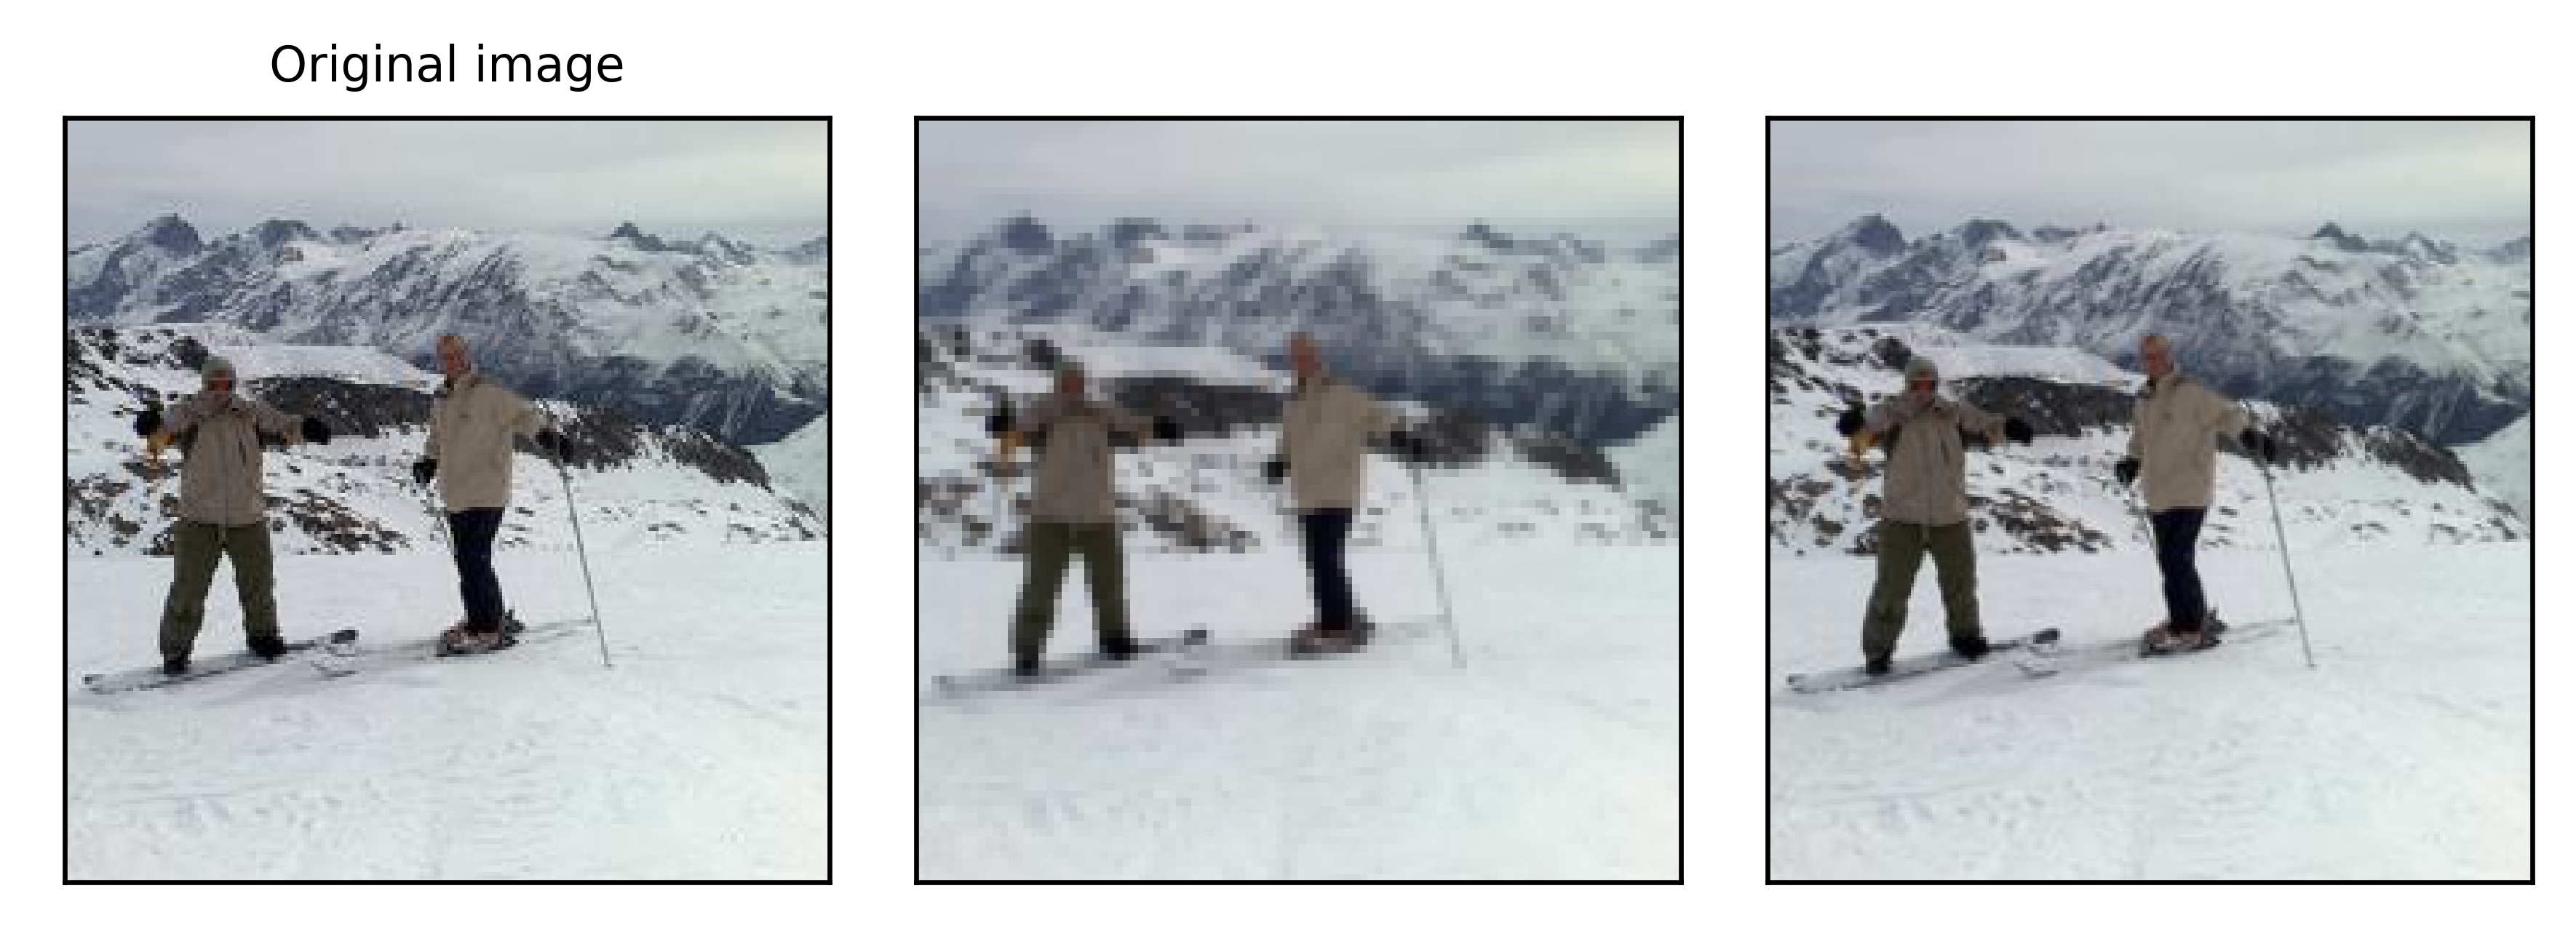
\includegraphics[scale=0.6]{Resize 1.2.png}}
\caption{Image After Being Resized}
\label{fig2}
\end{figure}

\paragraph{Random Cropping:}
Random Cropping means to randomly select and keep a certain fixed-sized zone of the image. We choose to create 3 probable $224\times224$-pixel cropping of each resized image ($256\times256$ pixels) presented as the subplot below on the far right\ref{fig3}, and the subplot in the middle is randomly cropped from a larger-sized image. 
\begin{figure}[H]  %用H做参数 强制固定图片位置
\centerline{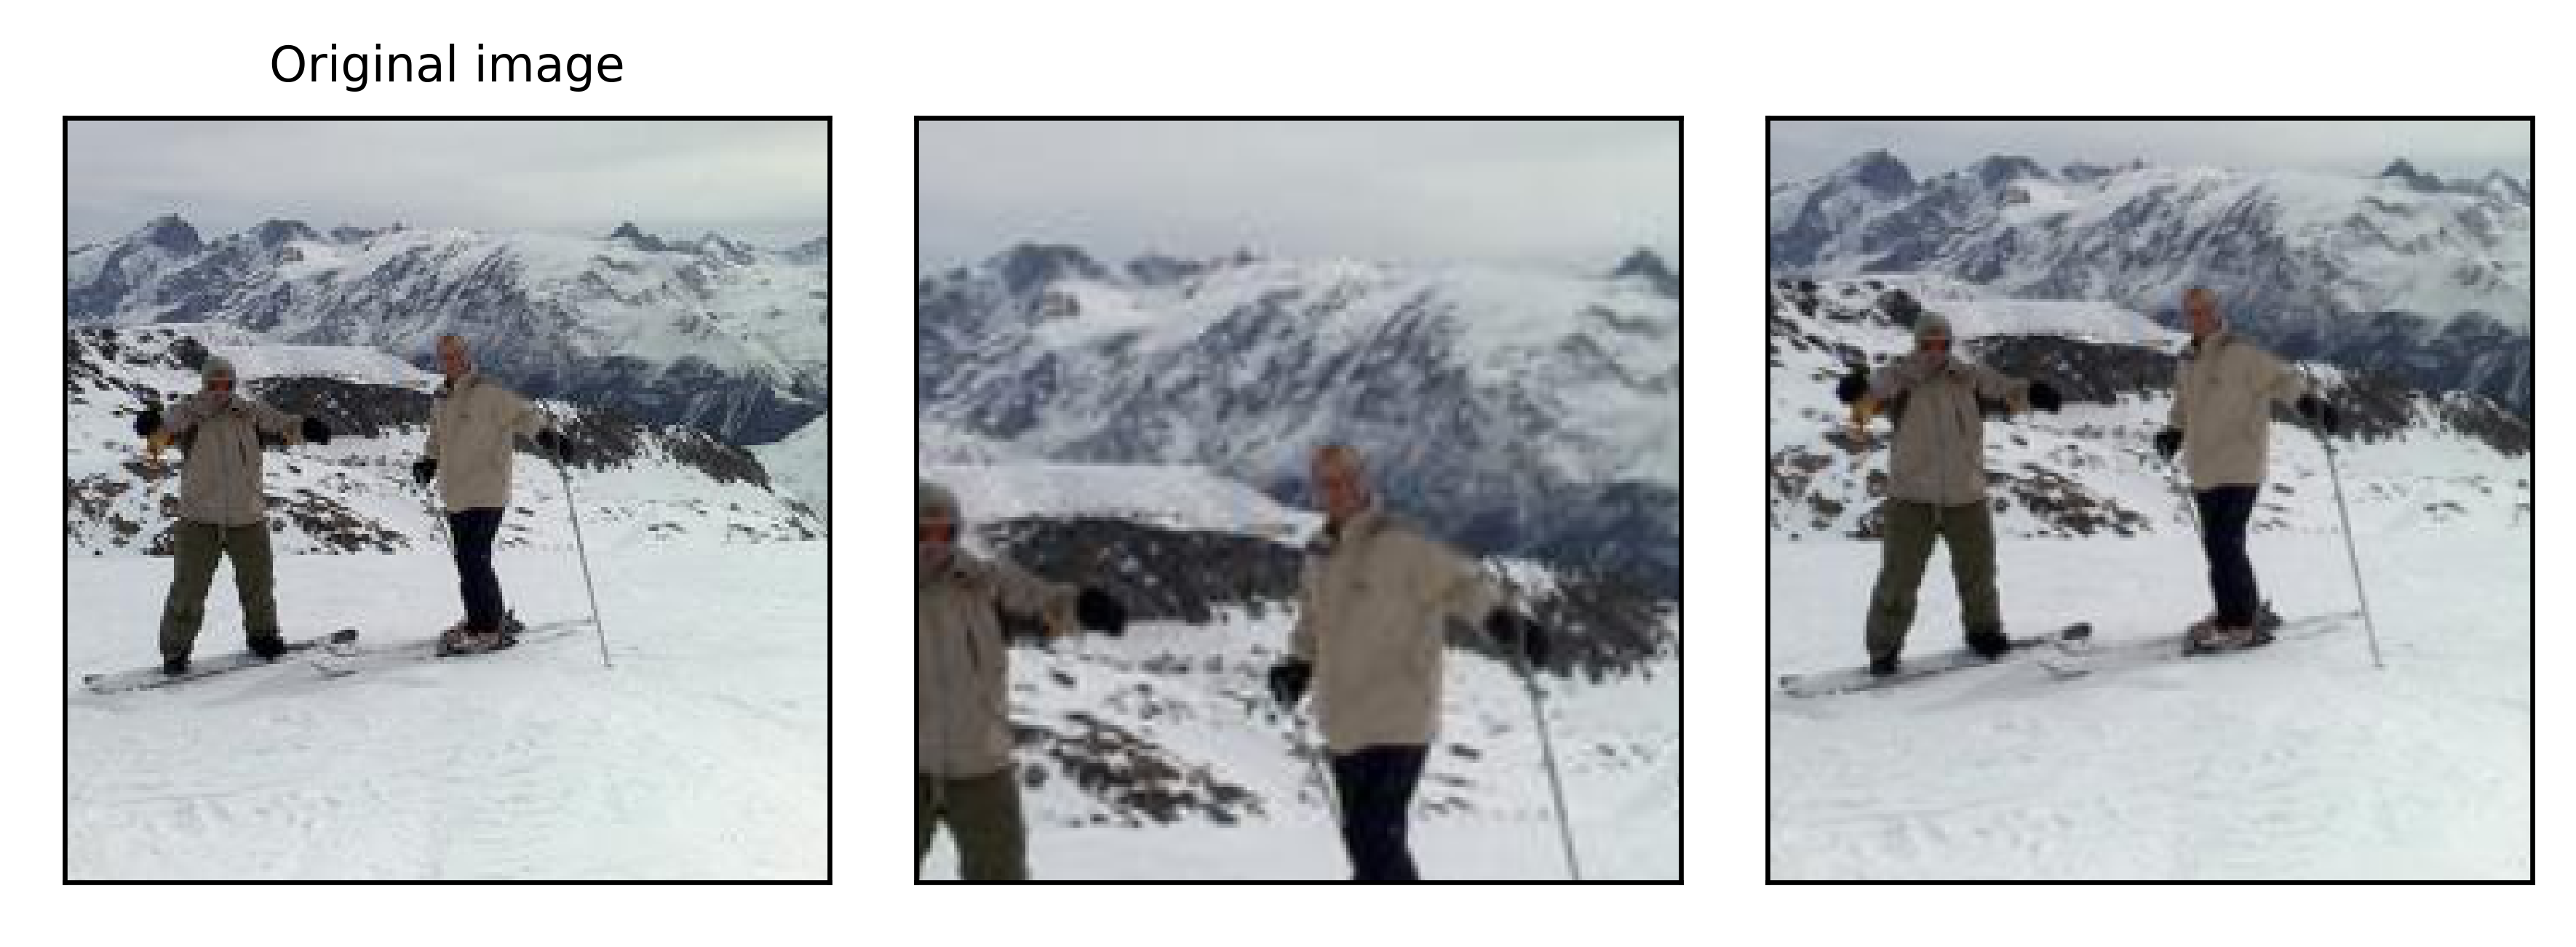
\includegraphics[scale=0.6]{Random Crop 1.1.png}}
\caption{Image After Being Randomly Cropped}
\label{fig3}
\end{figure}

\subsubsection{Random Horizontal/Vertical Flip}
Flipping the image horizontally or vertically can be easily completed by reversing the order of the pixels in each column or row of it, as shown in Figure \ref{fig4} and Figure \ref{fig5}.
\begin{figure}[H]
\centerline{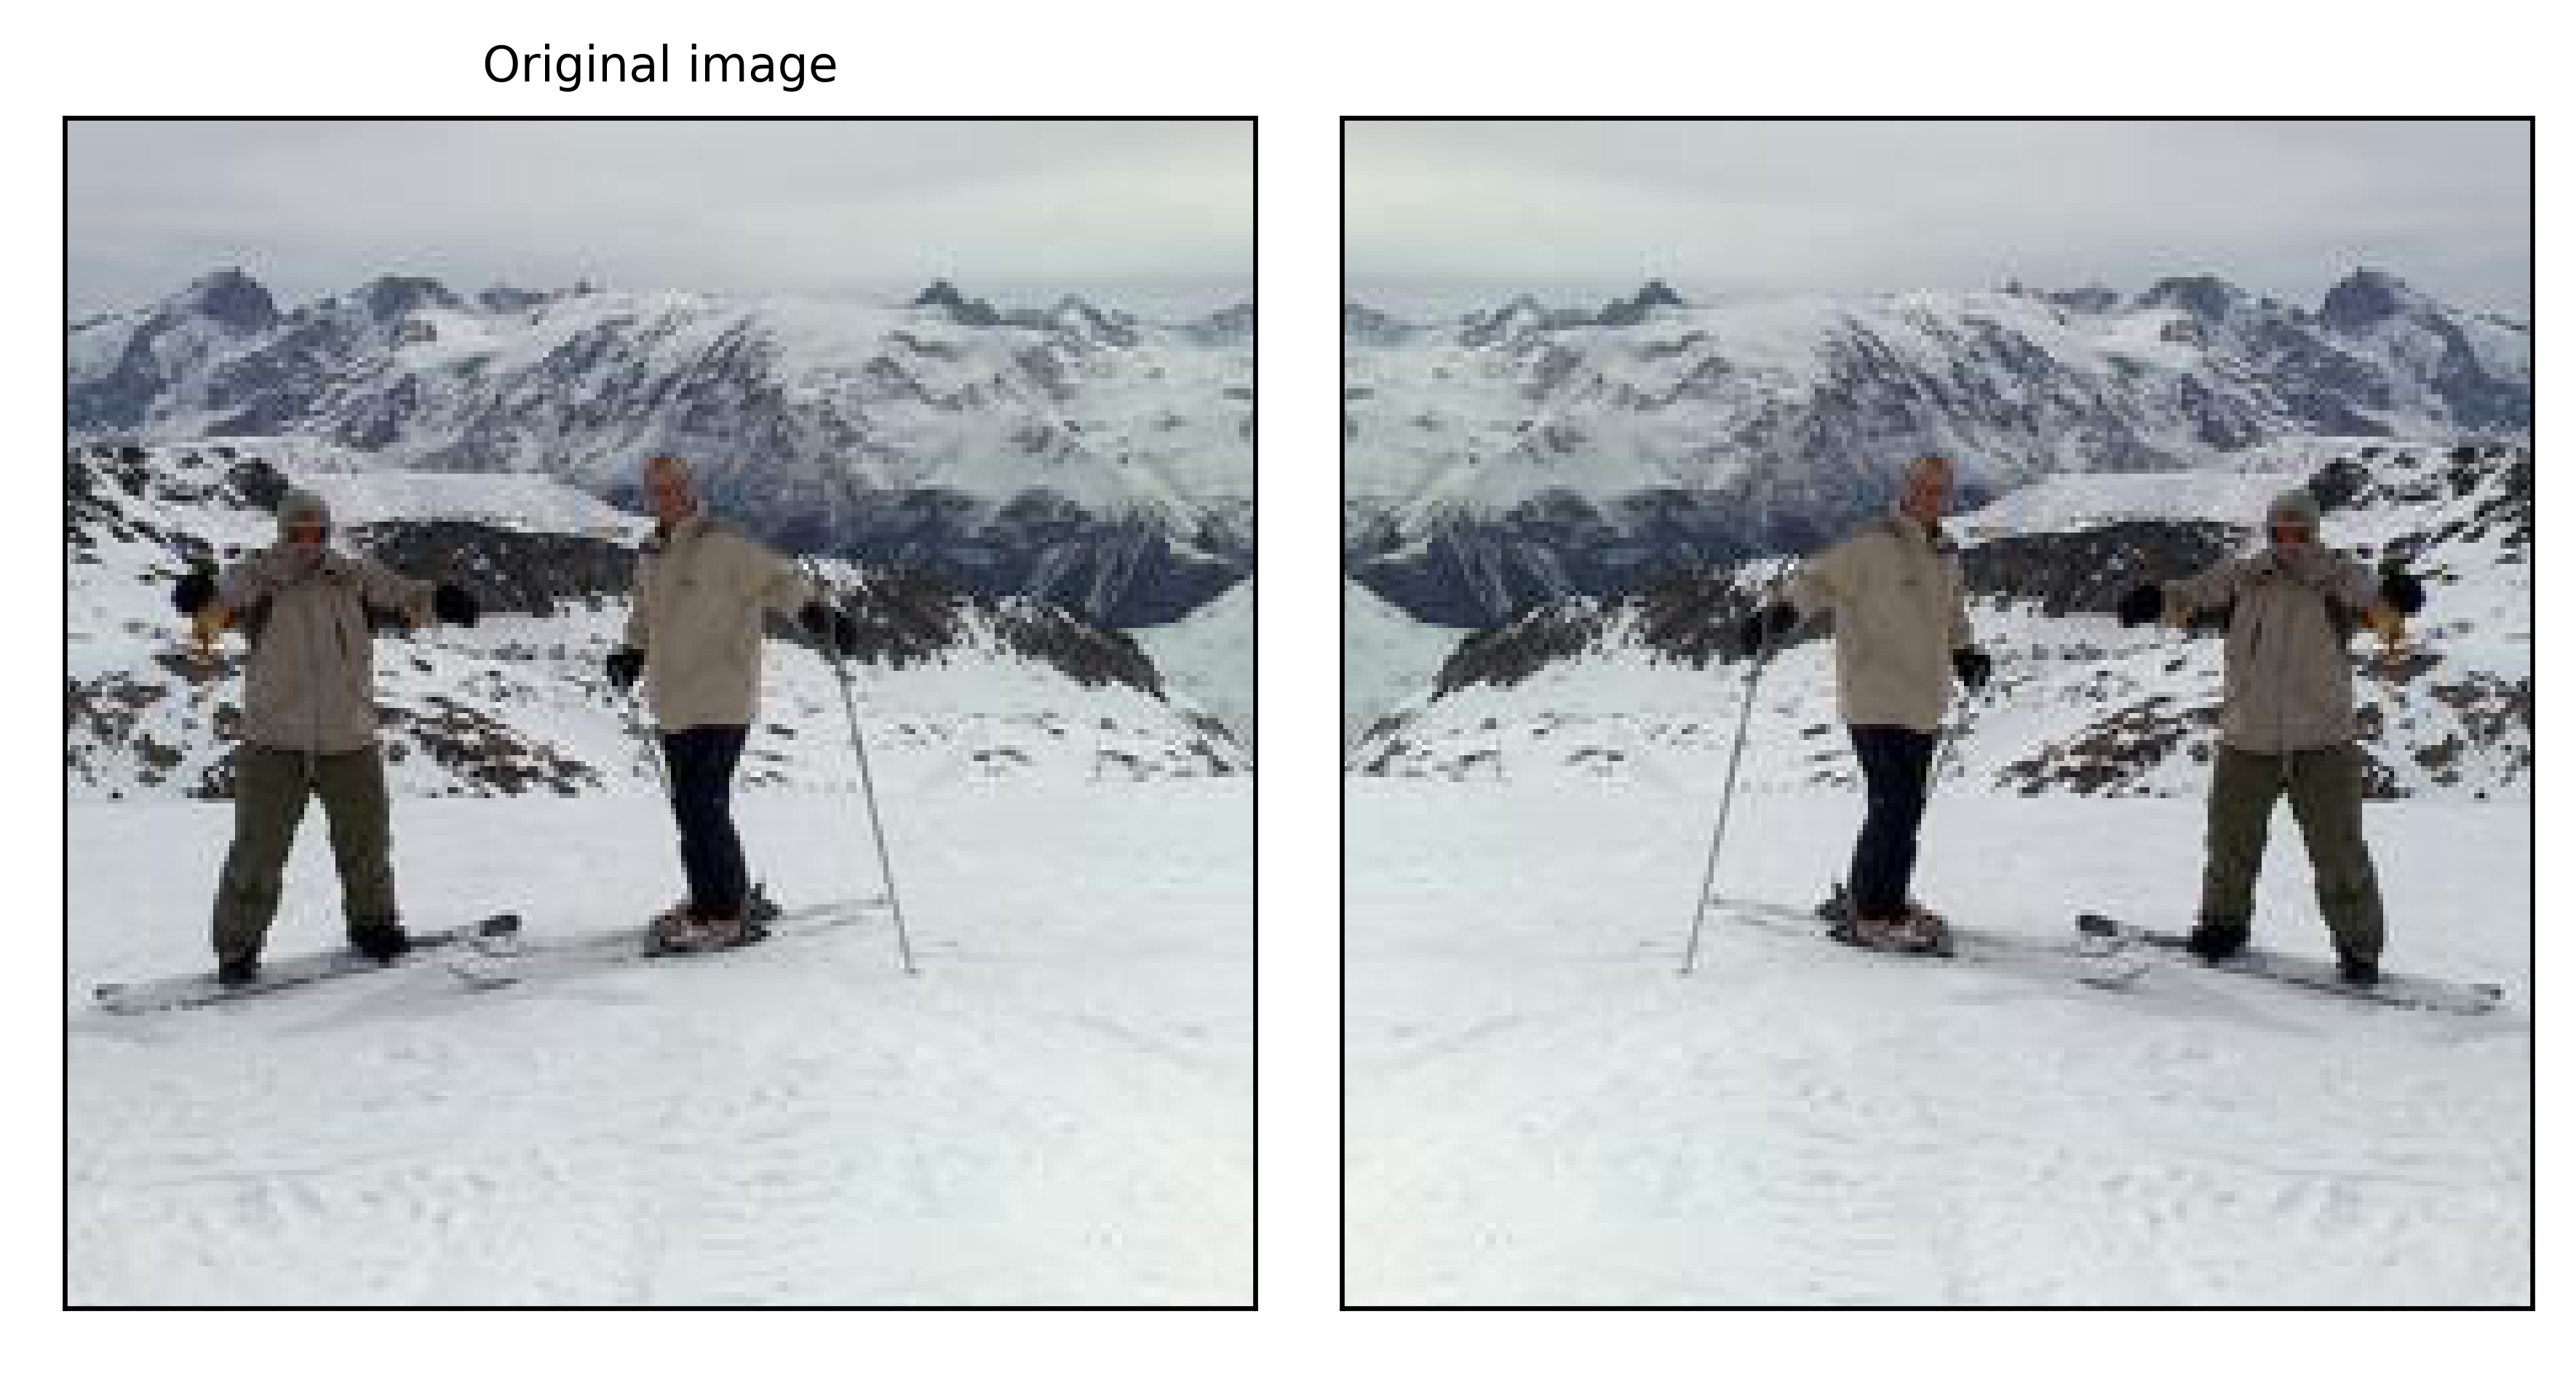
\includegraphics[scale=0.3]{Horizontal 1.0.png}}
\caption{Image After Being Horizontally Flipped}
\label{fig4}
\end{figure}
Representing the coordinate of one pixel in the flipped image as a vector of $(x,y)$:
\begin{equation}
f_{horizontal}((x,y))=(W-x,y), (x,y)\in image
\end{equation}
\begin{figure}[H]
\centerline{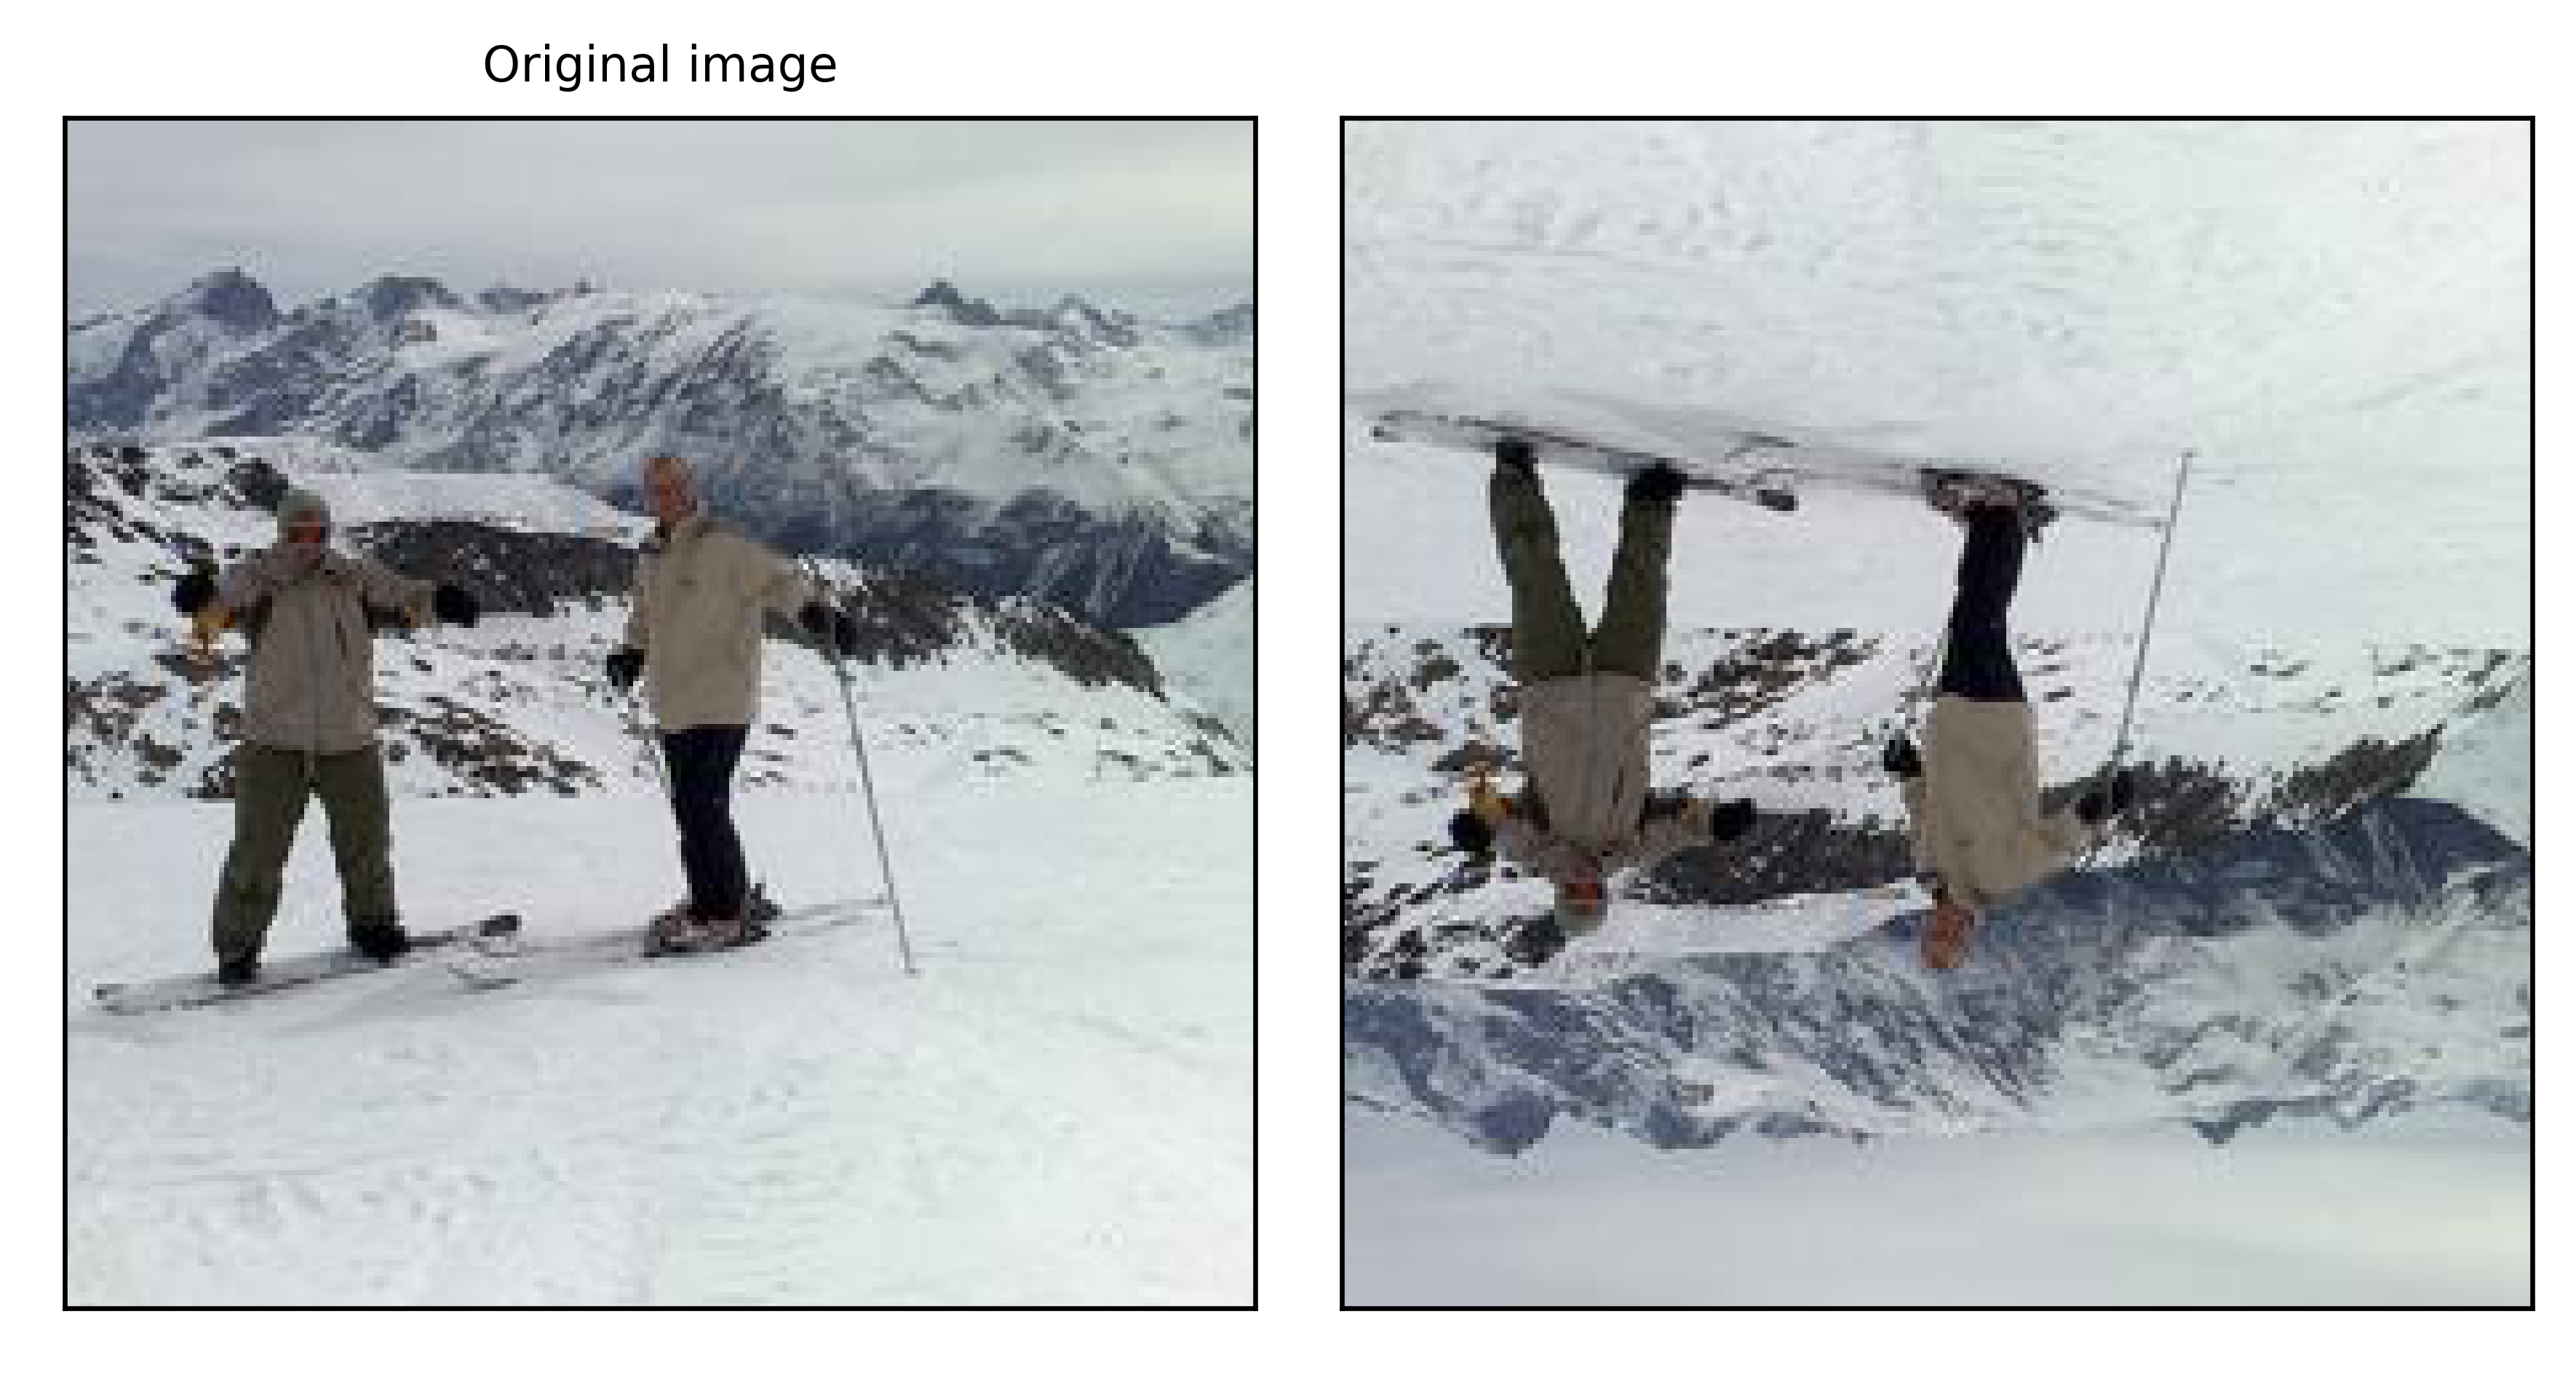
\includegraphics[scale=0.3]{Vertical 1.0.png}}
\caption{Image After Being Vertically Flipped}
\label{fig5}
\end{figure}
Similarly, we have:
\begin{equation}
f_{vertical}((x,y))=(x,H-y), (x,y)\in image
\end{equation}

\subsubsection{Random Rotation}
We also try to preprocess images by randomly rotating them at a certain angle in the range of [0\textdegree,45\textdegree], as visualized below.
\begin{figure}[H]
\centerline{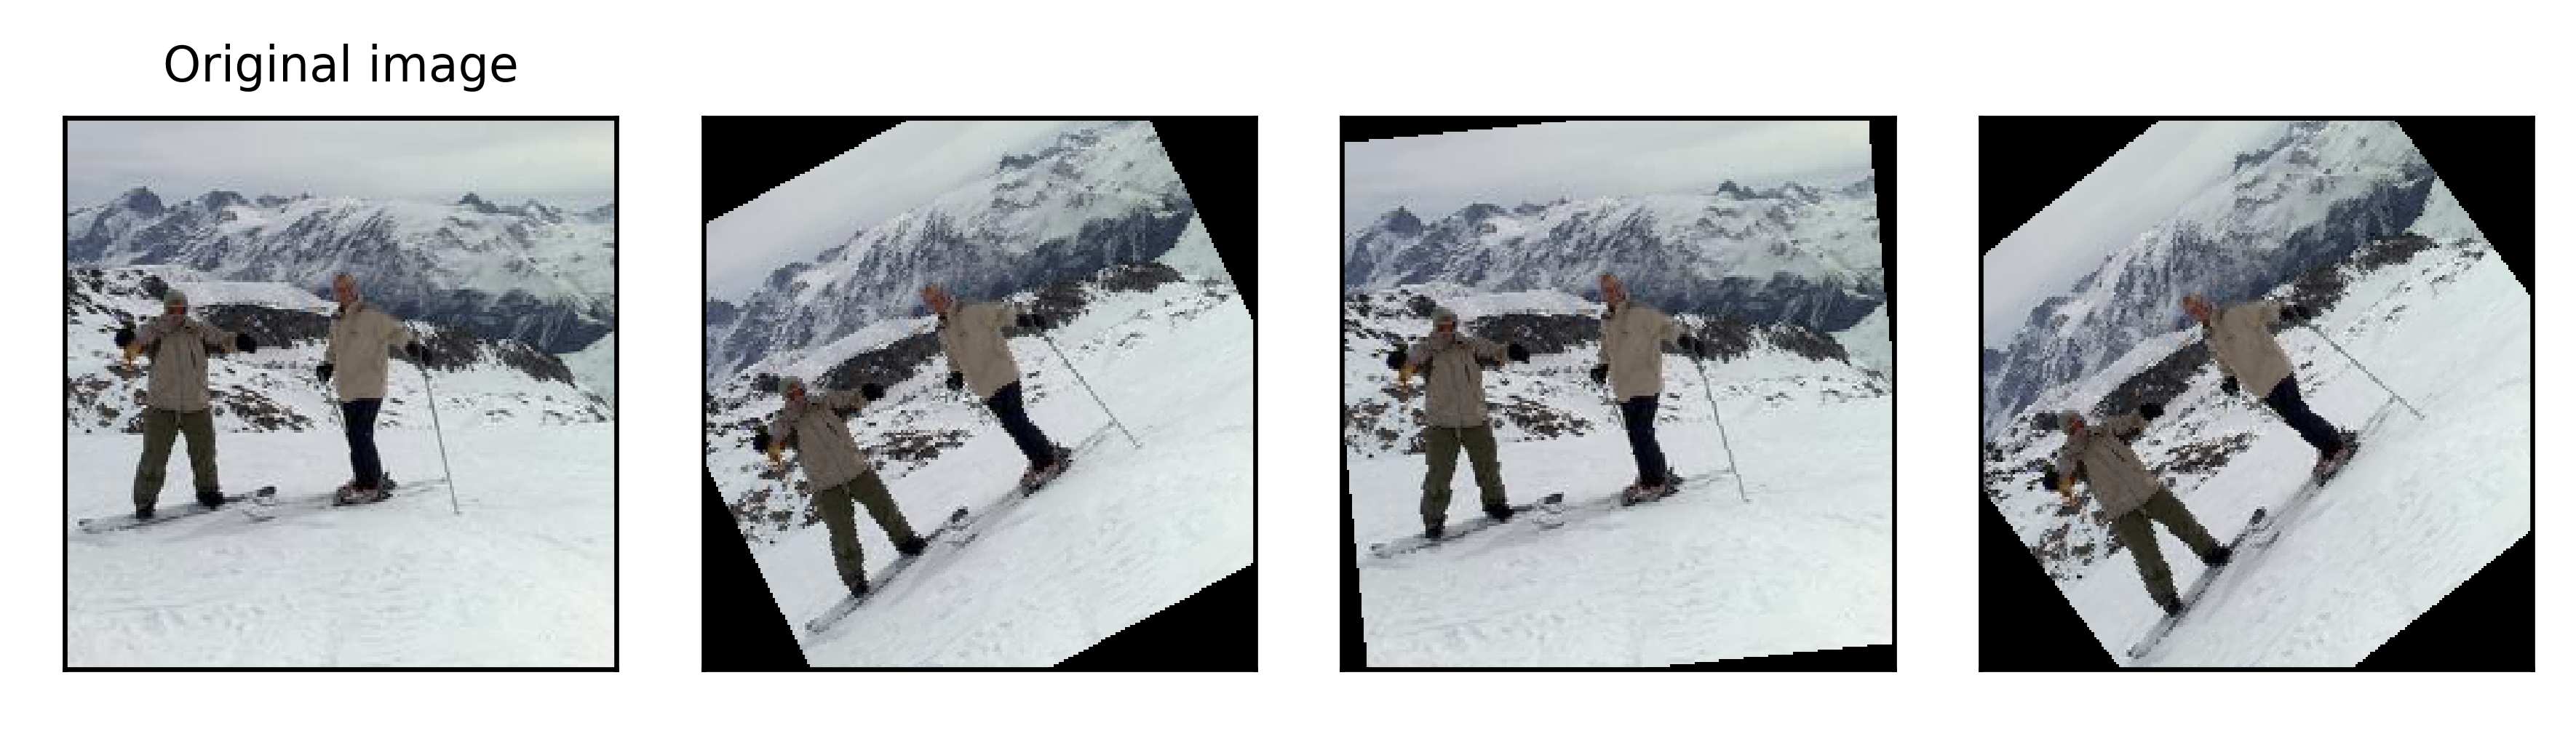
\includegraphics[scale=0.6]{Random rotate 1.0.png}}
\caption{Image After Being Randomly Rotated}
\label{fig6}
\end{figure}
It is evident that given the randomly generated angle $\theta$, the process of random rotation on the level of each pixel in the image can be expressed as:
\begin{multline}
f_{randomRotate}((x,y))=(xcos\theta-ysin\theta,xsin\theta+ycos\theta), \\(x,y)\in image
\end{multline}

\subsubsection{Random Affine}
The affine transformation consists of a linear transformation followed by a translation, and the equation of affine function is generalized in the form as below, limiting the rotation angle to [0\textdegree,45\textdegree] as well: 
\begin{multline}
f_{randomAffine}((x,y))=(A_1x+B_1y+\alpha,A_2x+B_2y+\beta),\\(x,y)\in image
\end{multline}

\begin{figure}[H]
\centerline{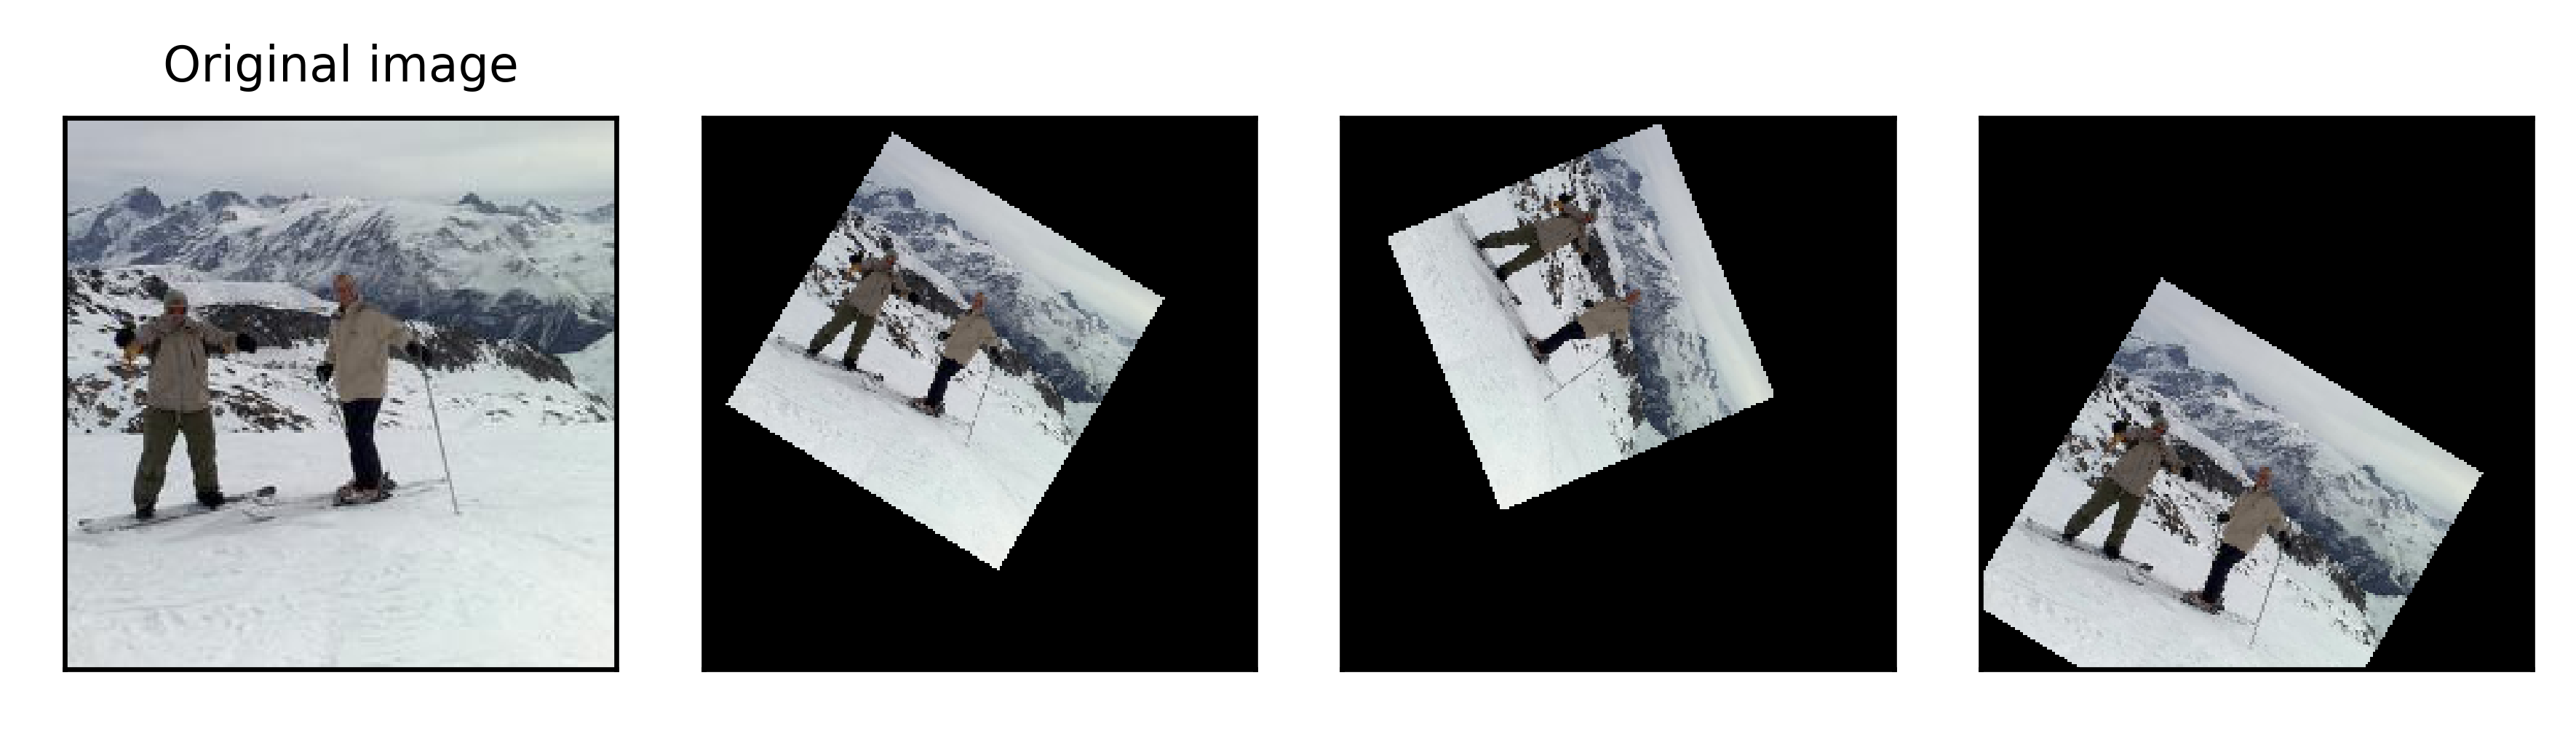
\includegraphics[scale=0.6]{Random Affine 1.0.png}}
\caption{Image After Being Randomly Affined}
\label{fig7}
\end{figure}

\subsubsection{Color Jitter}
\textbf{ColorJitter} is a type of image data augmentation where we randomly change the brightness, contrast and saturation of an image, as visualized in Figure \ref{fig8}


\begin{figure}[H]
\centerline{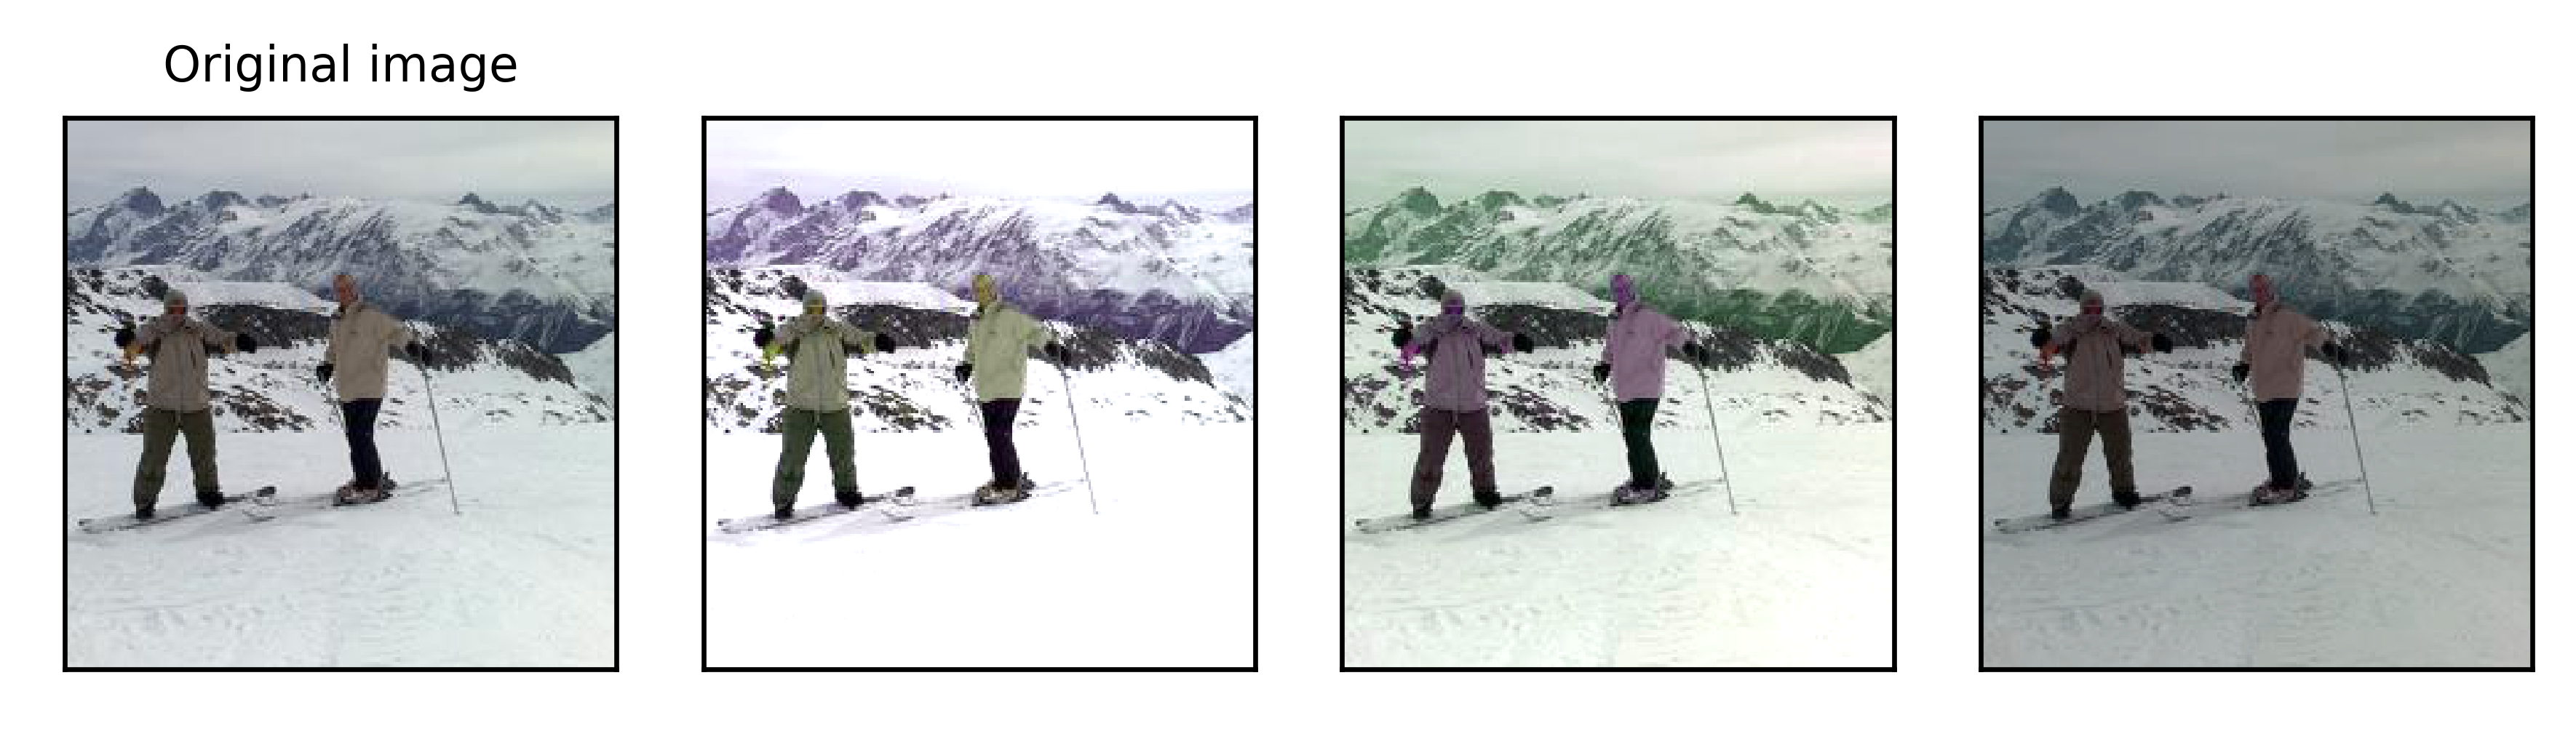
\includegraphics[scale=0.6]{Color Jitter 1.0.png}}
\caption{Image After Being Randomly Affined}
\label{fig8}
\end{figure}
\subsubsection{10-crop augmentation on test set}
To minimize the loss, 10-crop was employed as our test-time augmentation strategy. The entire process is divided into the following steps: 
\begin{enumerate}
    \item Since the reduced dataset was used for test, the size of each image has already been $224 \times 224$. To apply the crops properly, the test images will be first scaled up to $256 \times 256$. The size of the upsamples cannot be too large because we want to ensure that the latter crops should focus on the central part of the original image. 
    
    \item To apply 10-crop augmentation, the given image will be cropped into four corners and the central crop plus the horizontally flipped version of these cropped images, which is visualized in Figure \ref{10-crop}. In our case, 10 $224 \times 224$ images will be generated from the original version at the test stage. 
    
    \begin{figure}[htbp]
\centerline{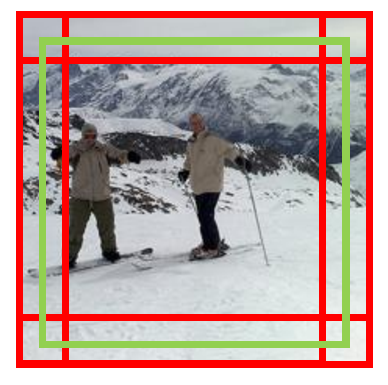
\includegraphics[scale=0.5]{10-crop.pdf}}
\caption{10-crop augmentation. Red squares refer to the crops at 4 corners, the green one is the center crop.}
\label{10-crop}
\end{figure}
    
    \item During the testing, multiple versions of each test image with fixed sizes were fed into the trained network. The loss and predictions across all variations are calculated and then averaged.
\end{enumerate}



\section{Experiments}
\label{sec:experiments}
\subsection{Experiment environment}
We use the pretrained ResNet-50 model as our transfer learning baseline. Loading the pretrained baseline weights could get 26\% accuracy on the given test data. However, we found that the pretrained model performs terribly on training data, with only 2\% or at best 3\% accuracy. We suspect that it is probable that the data used to train the baseline model is not consistent with the given training data. Overall, we trained the last fully connected layer of our model on the training data for 80 epochs, with the rest convolutional layers frozen. 

We have defined image transformation functions for both training data and test data. To apply the data augmentations methods to corresponding data, we use \textbf{ImageFolder} function to load training data and image transformation functions we defined previously. A custom data loader is used to load test data and corresponding transformation function. 
\subsection{Hyperparameters settings}
Since transfer learning method is applied, we should keep the hyperparameter of pretrained model unchanged and only use a small learning rate. The hyperparameter settings are showed in table\ref{tab:parameters}. The number of crops in validation set is 10 which takes a large amount of graphics memory and makes the training process slow, so we have to reduce the batch size to compensate for it. 

\begin{table}[htb]
\vskip 3mm
\begin{center}
\begin{small}
\begin{sc}
\begin{tabular}{lcccr}
\hline
Hyperparameter & value \\
\hline
Learning rate    & 0.01 \\
Dropout rate & 0.02\\
Batch size & 16\\
Image size & $224 \times 224$\\
Number of crops & 10\\
Number of epoch & 80\\

\hline
\end{tabular}
\end{sc}
\caption{Hyperparameter settings.}
\label{tab:parameters}
\end{small}
\end{center}
\vskip -3mm
\end{table}

\subsection{Train-Validation-Test Data Split}
The given training data was split into training data and validation data with splitting ratio of 9 : 1. The validation data is generated by randomly choosing 5 images for each category from the original training data and removing them into a new folder we created for validation data. Then the validation data loader is created through \textbf{ImageFolder} and the image transformation function we used is the same as test data. 

\subsection{Ablation study}
To validate our hyperparameters settings and methods applied in training the model, we carried out the ablation study using the following configurations: the model would be trained for 20 epochs with/without applying dropout/ten-crop while other hyperparameters settings are fixed. The testing results obtained after the 20th epoch are presented in Table \ref{tab:ablation}. It can be found that the model with dropout layer and test-time augmentation yields better performance than others. Therefore, such configuration would be used in the following experiments.

\begin{table}[h]
    \centering
    \begin{tabular}{|c|c|c|c|}
    \hline
     Dropout & Ten-crop & Test loss & Test acc \\
     \hline
     \checkmark & \checkmark & 4.4381 & 0.1785\\
      \hline
     \text{\sffamily X} & \checkmark & 4.5976 & 0.1762\\
      \hline
     \checkmark & \text{\sffamily X}  & 4.6297 & 0.1707\\
      \hline
     \text{\sffamily X} & \text{\sffamily X} & 4.6765 & 0.1758\\
     \hline
    \end{tabular}
    \caption{Results obtained after the 20 epochs training. \\
    \checkmark \& \text{\sffamily X} indicates whether the method is applied or not.}
    \label{tab:ablation}
\end{table}


\subsection{Experiment results}

We trained our model for 80 epochs in total, and after every 20 epoch we tested our model on the test data. Figure\ref{train} shows the error and accuracy of training and validation data. According to this figure, we could find out that the training accuracy is extremely low at the beginning of the training process, while the validation accuracy is more than 10\%, which is obviously much higher than training accuracy. As training proceeds, the training error decreases rapidly and becomes smooth after the 30th epoch. There is not much improvement on the validation error since its accuracy increases from 15.42\% at epoch 5 to 19.56\% at epoch 80, while the training accuracy reaches 22.03\%. 

\begin{figure}[H]
\centerline{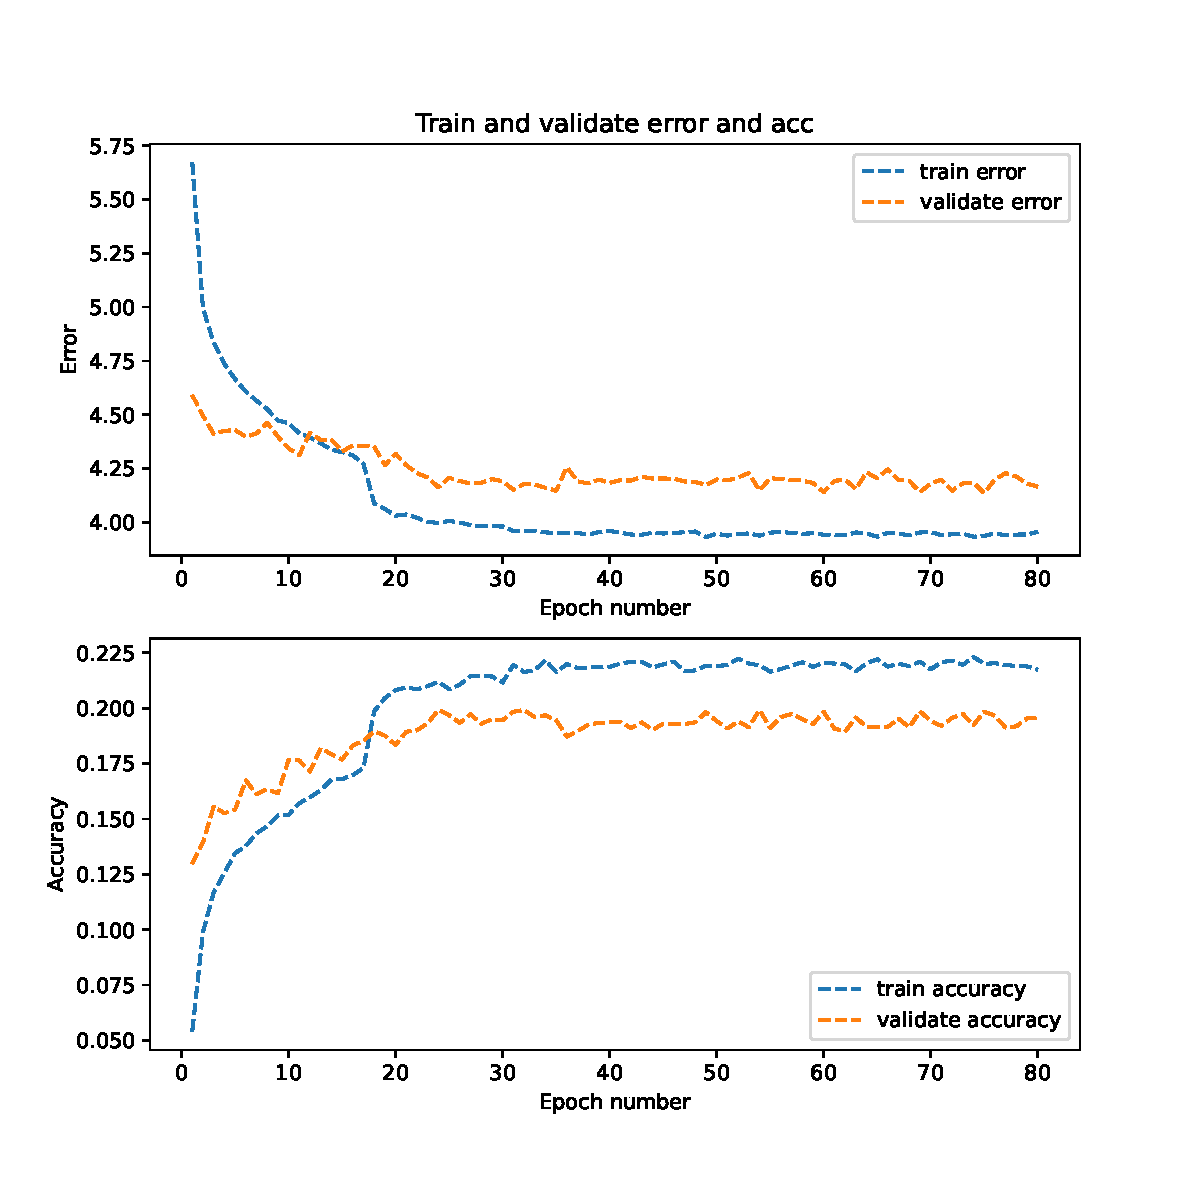
\includegraphics[scale=0.4]{train.pdf}}
\caption{Error and accuracy for train and validate data}
\label{train}
\end{figure}

Figure\ref{test} shows the error and accuracy of test data at epoch 20, 40, 60, 80 respectively. There is a clear improvement on test accuracy before 40 epoch and the performance of the model reaches its maximum at the 60th epoch with accuracy of 19.2\% and loss of 4.3\%. After 60 epochs, the accuracy decreases slightly because there might be an overfitting problem. Overall, our results on the test data are that the accuracy is capped at 20\% no matter how many epochs we trained afterwards. 


\begin{figure}[H]
\centerline{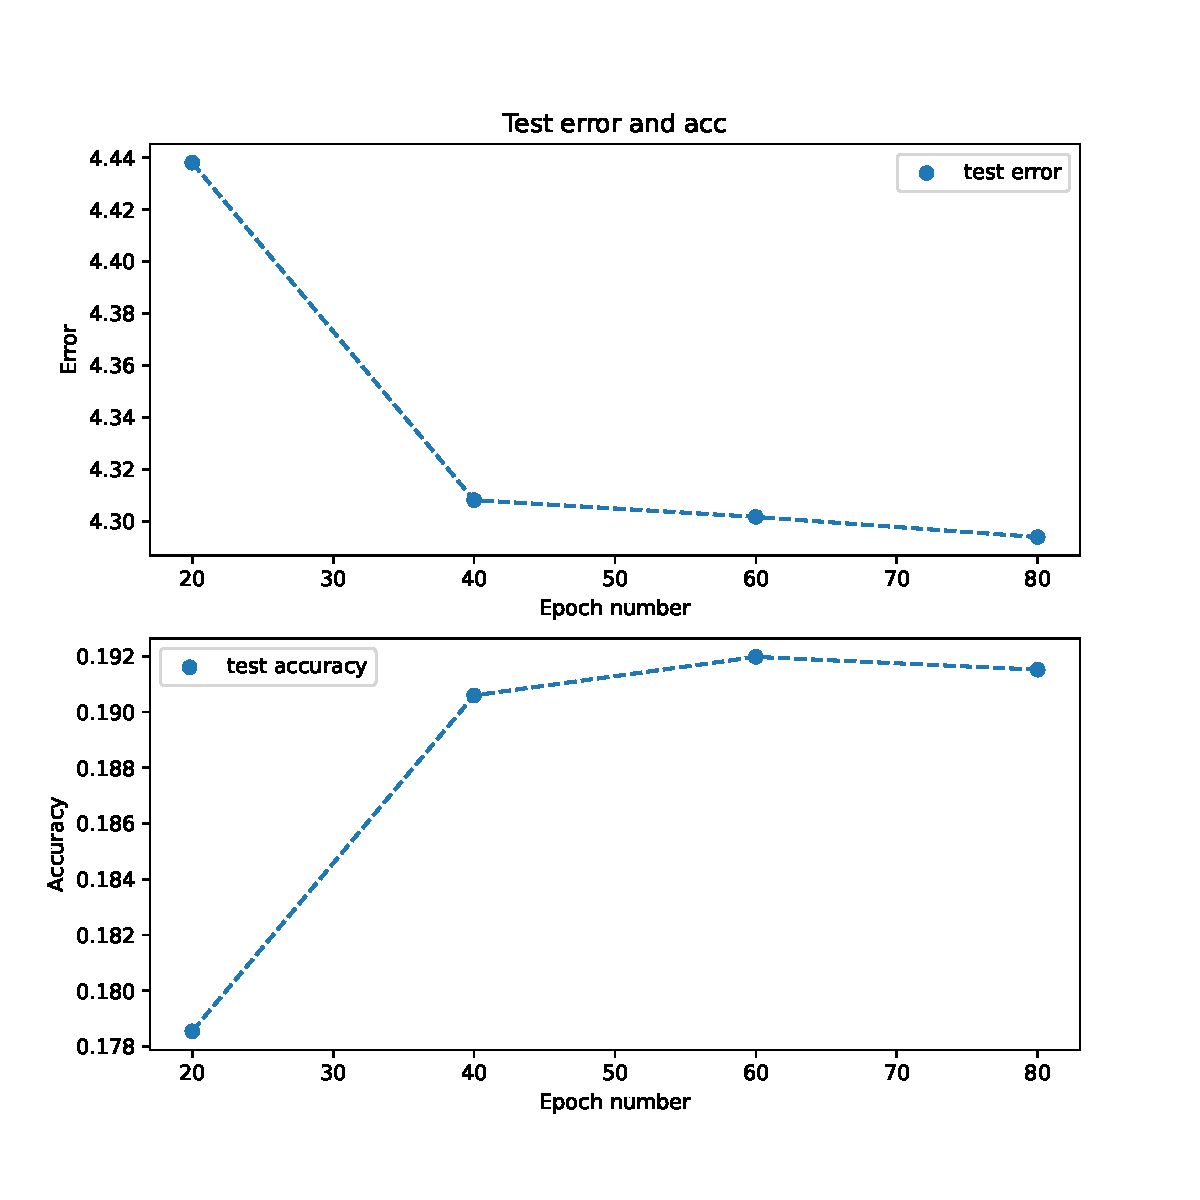
\includegraphics[scale=0.4]{test.pdf}}
\caption{Error and accuracy for test data}
\label{test}
\begin{small}
\end{small}
\end{figure}

\subsection{Class-wise performance analysis}
After evaluating the best model we got, the top-6 classes with highest F1-score are listed in Table \ref{tab:top6}. The class 'jacamar' had the best F1 score which is 0.8. Additionally, the class 'yellow\_lady’s\_slipper' had the highest true positive rate where 45 out of 50 test images were predicted correctly.  

As for the classes with the worst performance, 81 classes had 0 true positive rate which means none of the images in these classes were classified correctly. 

\begin{table}[h]
\resizebox{\linewidth}{!}{
\begin{tabular}{|r|r|r|r|r|}
\hline
\multicolumn{1}{|l|}{\textbf{\#}} & \multicolumn{1}{l|}{\textbf{Class Name}} & \multicolumn{1}{l|}{\textbf{precision}} & \multicolumn{1}{l|}{\textbf{recall}} & \multicolumn{1}{l|}{\textbf{f1-score}} \\ \hline
95                                & jacamar                                  & 0.79                                    & 0.82                                 & 0.8                                    \\ \hline
139                               & ruddy\_turnstone                         & 0.68                                    & 0.78                                 & 0.73                                   \\ \hline
986                               & yellow\_lady's\_slipper                  & 0.54                                    & 0.9                                  & 0.68                                   \\ \hline
392                               & rock\_beauty                             & 0.62                                    & 0.74                                 & 0.67                                   \\ \hline
251                               & dalmatian                                & 0.67                                    & 0.66                                 & 0.67                                   \\ \hline
24                                & great\_grey\_owl                         & 0.72                                    & 0.62                                 & 0.67                                   \\ \hline
\end{tabular}
}
\caption{Top-6 F1 scores}
\label{tab:top6}
\end{table}

Besides, we also investigated the most confusing pairs of classes for the trained ResNet-50, where the model has a larger probability of misclassifying one class as the other. Some samples are picked from training data and shown in Table \ref{tab:pairs}. For these classes, it can be observed that the images in each pair have similar patterns, which are difficult to distinguish from each other, even for human beings. 

\begin{table}[]
    \centering
    \begin{tabular}{|c c|}
    \hline
    jaguar   &  leopard\\
    \begin{minipage}{.4\linewidth}
    \centering
      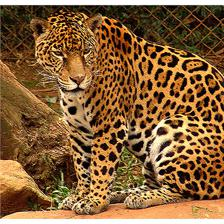
\includegraphics[width=.6\linewidth]{pairs/jaguar.JPEG}
    \end{minipage}     & 
    \begin{minipage}{.4\linewidth}
    \centering
      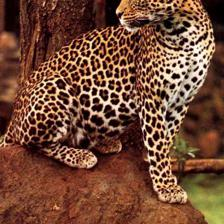
\includegraphics[width=.6\linewidth]{pairs/leopard.JPEG}
    \end{minipage}\\
        \hline
    silky\_terrier   &  yorkshire\_terrier\\
    \begin{minipage}{.4\linewidth}
    \centering
      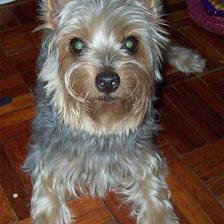
\includegraphics[width=.6\linewidth]{pairs/silky_terrier.JPEG}
    \end{minipage}     & 
    \begin{minipage}{.4\linewidth}
    \centering
      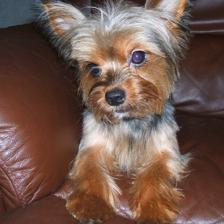
\includegraphics[width=.6\linewidth]{pairs/Yorkshire_terrier.JPEG}
    \end{minipage}\\
        \hline
    trolleybus   &  streetcar\\
    \begin{minipage}{.4\linewidth}
    \centering
      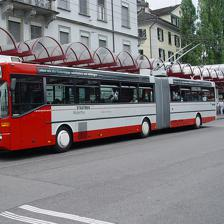
\includegraphics[width=.6\linewidth]{pairs/trolleybus.JPEG}
    \end{minipage}     & 
    \begin{minipage}{.4\linewidth}
    \centering
      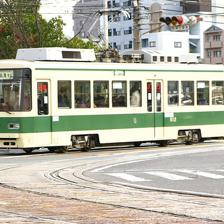
\includegraphics[width=.6\linewidth]{pairs/streetcar.JPEG}
    \end{minipage}\\
     \hline
    \end{tabular}
    \caption{Confusing pairs of images}
    \label{tab:pairs}
\end{table}



\section{Related work}
\label{sec:relwork}
In literature exists some approach for the VIPriors Image Classification Challenge. The team from Alibaba Group achieved the first place in this competition with the Dual Selective Kernel (DSK) network\cite{sun2020visual}, which reached 75.5\% as the top-1 accuracy. The proposed network employed several expert models in parallel with the same initial layers but different classifiers. The model architecture is shown in Figure \ref{alibaba}. Each of the classifier optimises against distilled targets generated by the teacher model. The final prediction would be based on the average fusion results of all the expert models. 

\begin{figure}[H]
\centerline{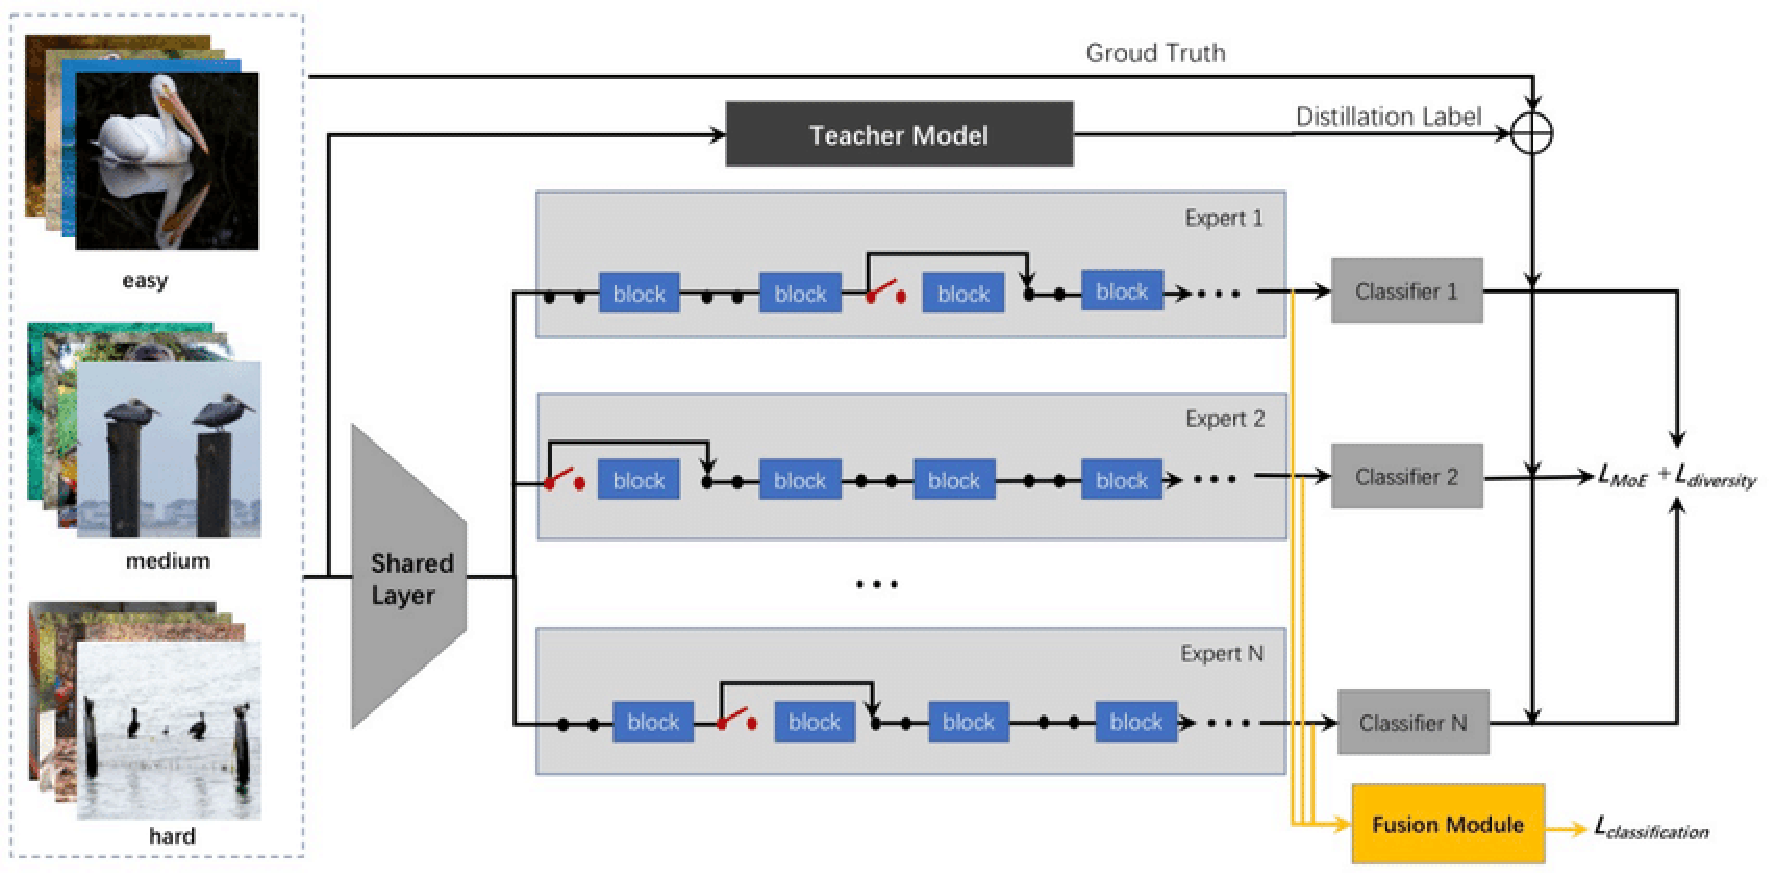
\includegraphics[scale=0.25]{alibaba.pdf}}
\caption{Dual Selective Kernel(DSK) network\cite{lengyel2022vipriors}}
\label{alibaba}
\end{figure}

The DeepBlueAI team utilized recent image augmentation methods and ensemble learning to improve the models’ robustness and generalization. Three models including ResNest101\cite{zhang2020resnest}, TResNet-XL\cite{ridnik2021tresnet} and SEResNeXt101\cite{hu2018squeeze} were used as backbones. After the models was well trained, the test accuracy based on fused model predictions achieved 70.15\% \cite{luo2020technical}.

Another team from Friedrich Schiller University Jena and Sapienza University of Rome used ResNeXt-101\cite{xie2017aggregated} as the model structure. Besides standard techniques of data augmentation, they also applied test-time augmentation, where each test image would generate 30 variants with the size range from 256 to 352. 20 independently trained ResNeXt-101 models are aggregating as their final predictions, which yielded 69.7\% test accuracy on the given dataset\cite{barz2021strong}.


\section{Conclusions}
\label{sec:concl}
% this is conclusion 
Based on various methods involving data augmentation and frozen layers, we have managed to complete the image classification task, achieving an accuracy of 20\%, higher than the initial 2 $\sim$ 3\% accuracy obtained at the beginning.

Since we did not successfully outperform the given baseline model accuracy (31\%) as specified in the Vipriors challenges, future work may include increasing training epochs, adjusting the loss function, applying contrastive learning\cite{khosla2020supervised} and ensemble learning to achieve better performance.



% 引用区

\bibliographystyle{plain} % We choose the "plain" reference style
\bibliography{example-refs} % Entries are in the refs.bib file

\onecolumn
\section{Appendix}
\textbf{Acknowledgement: The experiments are based in parts on code and text kindly provided by Herick Asmani\footnote{https://github.com/Herick-Asmani/Food-101-classification-using-ResNet-50}.}


\subsection{Imports}
\begin{minted}
[
baselinestretch=1.2,
fontsize=\normalsize,
linenos,
breaklines
]
{python}
import numpy as np # linear algebra
import pandas as pd # data processing, CSV file I/O (e.g. pd.read_csv)
import os
from PIL import Image
from collections import OrderedDict
from tqdm import tqdm

# Import necessary PyTorch libraries
import torch
from torch import nn
from torch import optim
import torch.nn.functional as F
from torch.utils.data import DataLoader
from torchvision.models import resnet50
from torchvision import datasets, transforms, models
\end{minted}
\subsection{Generating Validation Set}
\begin{minted}
[
baselinestretch=1.2,
fontsize=\normalsize,
linenos,
breaklines
]
{python}
import shutil
# generate validate set
if not os.path.exists('ImageNet/validate'):
    os.mkdir('ImageNet/validate')
rootdir = 'ImageNet/train'
list=os.listdir(rootdir)
for cls in list:
    path = os.path.join(rootdir, cls)
    des_path = os.path.join('ImageNet/validate', cls)
    if not os.path.exists(des_path):
        os.mkdir(des_path)
    for idx, item in enumerate(os.listdir(path)):
        full_path = os.path.join(path, item)
        if len(os.listdir(des_path)) < 5:
            shutil.move(full_path,des_path)
\end{minted}
\subsection{Data preprocessing}
\begin{minted}
[
baselinestretch=1.2,
fontsize=\normalsize,
linenos,
breaklines
]
{python}
class CustomDataset(torch.utils.data.Dataset):

    def __init__(self, img_path, labels, transform=None):
        self.path = img_path
        self.data_paths = [f for f in os.listdir(img_path)]
        self.labels = labels
        self.transform = transform

    def __getitem__(self, idx):
        img = Image.open(os.path.join(self.path,self.data_paths[idx]))
        img = img.convert("RGB")
        label = self.labels[idx]
        if self.transform:
            img = self.transform(img)
        
        return img, label

    def __len__(self):
        return len(self.data_paths)
        
##############Data Augumentation ###########################
train_transforms = transforms.Compose([transforms.RandomHorizontalFlip(),
                                       transforms.RandomVerticalFlip(),
                                       transforms.RandomRotation(45),
                                       transforms.RandomAffine(45),
                                       transforms.ColorJitter(),
                                       transforms.ToTensor(),
                                       transforms.Normalize(mean=[0.485, 0.456, 0.406],
                                                            std=[0.229, 0.224, 0.225])])

####################################################################

test_transforms = transforms.Compose([transforms.Resize(256),
                                      transforms.TenCrop(224),
                                      transforms.Lambda(lambda crops: torch.stack([transforms.ToTensor()(crop) for crop in crops])),
                                      transforms.Lambda(lambda crops: torch.stack([transforms.Normalize(mean=[0.485, 0.456, 0.406],std=[0.229, 0.224, 0.225])(crop) for crop in crops]))])
test_transforms_no_crop = transforms.Compose([transforms.Resize((224, 224)),
                                transforms.RandomHorizontalFlip(), 
                                transforms.ToTensor(),
                                transforms.Normalize((0.485, 0.456, 0.406), (0.229, 0.224, 0.225))])

#for ablation study
no_crop = True
no_dropout = False

train_dir = 'ImageNet/train'
train_data = datasets.ImageFolder(train_dir, train_transforms)

val_dir = 'ImageNet/validate'
validate_data = datasets.ImageFolder(val_dir, test_transforms)

test_dir = 'ImageNet/test'
if no_crop:
    test_data = CustomDataset(test_dir,test_label,test_transforms_no_crop)
else:
    test_data = CustomDataset(test_dir,test_label,test_transforms)
    
batch_size = 16
dataloaders = {}
dataloaders['train'] = DataLoader(train_data, batch_size=batch_size, shuffle=True)
dataloaders['validate'] = DataLoader(validate, batch_size=batch_size, shuffle=False)
dataloaders['test'] = DataLoader(test, batch_size=batch_size, shuffle=False)

load_baseline = False
continue_train = True

model = resnet50(pretrained=False)
if load_baseline:
    checkpoint = torch.load('ImageNet/resnet50_fconv_model_best.pth.tar')
    print('Load from baseline')
    new_state_dict = OrderedDict()
    for k, v in checkpoint['state_dict'].items():
        name = k[7:] # remove module.
        new_state_dict[name] = v

    model.load_state_dict(new_state_dict)
    if not no_dropout:
        print('dropout')
        model.fc = nn.Sequential(nn.BatchNorm1d(2048), nn.Dropout(0.2), nn.Linear(2048, 1000))
        
        
sum(p.numel() for p in model.parameters() if p.requires_grad)

ct = 0
for child in model.children():
  ct += 1
  if ct < 10:
      for param in child.parameters():
          param.requires_grad = False
          
sum(p.numel() for p in model.parameters() if p.requires_grad)

if continue_train:
    train_on_gpu = torch.cuda.is_available()
    print('Load from checkpoint')
    checkpoint = torch.load('ImageNet/res50_model_checkpoint.pth', map_location=torch.device('cuda'))
    model = checkpoint['model']
    criterion = checkpoint['criterion']
    optimizer = optim.SGD(model.parameters(), lr=0.01)
    scheduler = torch.optim.lr_scheduler.ReduceLROnPlateau(optimizer, 'min', patience = 5)
    n_epochs = 20
    valid_loss_min = checkpoint['valid_loss_min'] # track change in validation loss
else:
    # specify loss function (categorical cross-entropy)
    criterion = nn.CrossEntropyLoss()

    # specify optimizer (stochastic gradient descent with momentum)
    optimizer = optim.SGD(model.parameters(), lr=0.01)

    # secify learning rate scheduler (if there is no further decrease in loss for next 5 epochs 
    # then lower the learning rate by 0.1)
    scheduler = torch.optim.lr_scheduler.ReduceLROnPlateau(optimizer, 'min', patience = 5)

    train_on_gpu = torch.cuda.is_available()
    # Move the model to GPU if CUDA is available
    if train_on_gpu:
        model.cuda()

    # number of epochs to train the model
    n_epochs = 20

    valid_loss_min = np.Inf # track change in validation loss
\end{minted}

\subsection{Model Training and Testing}
\begin{minted}
[
baselinestretch=1.2,
fontsize=\normalsize,
linenos,
breaklines
]
{python}
train_error = {}
train_acc = {}
validate_error = {}
validate_acc = {}
for epoch in range(cur_epochs, n_epochs+1):
    # keep track of training and validation loss
    
    train_loss = 0.0
    train_accuracy = 0.0
    valid_loss = 0.0
    val_accuracy = 0.0
    

    ###################
    # train the model #
    ###################
    loop = tqdm(enumerate(dataloaders['train']),total=len(dataloaders['train']))
    model.train()
    for batch_idx, (data, target) in loop:
        
        # move tensors to GPU if CUDA is available
        if train_on_gpu:
            data, target = data.cuda(), target.cuda()
        # clear the gradients of all optimized variables
        optimizer.zero_grad()
        # forward pass: compute predicted outputs by passing inputs to the model
        output = model(data)
        # calculate the batch loss
        loss = criterion(output, target)
        # backward pass: compute gradient of the loss with respect to model parameters
        loss.backward()
        # perform a single optimization step (parameter update)
        optimizer.step()
        # update training loss
        train_loss += loss.item()*data.size(0)
        # Calculate training accuracy
        top_p, top_class = output.topk(1, dim=1)
        equals = top_class == target.view(*top_class.shape)
        train_accuracy += torch.mean(equals.type(torch.FloatTensor)).item()*data.size(0)
        
        loop.set_description(f'train Epoch[{epoch}/{n_epochs}]')
        loop.set_postfix(loss=train_loss/len(dataloaders['train'].dataset), acc=train_accuracy/((batch_idx+1)*batch_size))
        
        
        
    ######################    
    # validate the model #
    ######################
    loop = tqdm(enumerate(dataloaders['validate']),total=len(dataloaders['validate']),leave=False)
    model.eval()
    with torch.no_grad():
        for batch_idx, (data, target) in loop:
            # move tensors to GPU if CUDA is available
            if train_on_gpu:
                data, target = data.cuda(), target.cuda()

            input_var = torch.autograd.Variable(data, volatile=True)
            target_var = torch.autograd.Variable(target, volatile=True)
            bs, ncrops, c, h, w = input_var.size()
            # forward pass: compute predicted outputs by passing inputs to the model
            temp_output = model(input_var.view(-1, c, h, w))
            output = temp_output.view(bs, ncrops, -1).mean(1)
            # calculate the batch loss
            loss = criterion(output, target_var)
            # update average validation loss 
            valid_loss += loss.item()*data.size(0)
            # Calculate validation accuracy
            top_p, top_class = output.topk(1, dim=1)
            equals = top_class == target.view(*top_class.shape)
            val_accuracy += torch.mean(equals.type(torch.FloatTensor)).item()*data.size(0)
            
            loop.set_description(f'validate Epoch[{epoch}/{n_epochs}]')
            loop.set_postfix(loss=valid_loss/len(dataloaders['validate'].dataset), acc=val_accuracy/((batch_idx+1)*batch_size))
            
    
    # calculate average losses and accuracies
    train_loss = train_loss/len(dataloaders['train'].dataset)
    train_accuracy = train_accuracy/len(dataloaders['train'].dataset)
    valid_loss = valid_loss/len(dataloaders['validate'].dataset)
    val_accuracy = val_accuracy/len(dataloaders['validate'].dataset)
    
    train_error[epoch] = train_loss
    train_acc[epoch] = train_accuracy
    validate_error[epoch] = valid_loss
    validate_acc[epoch] = val_accuracy
    
    # Learning rate scheduler step
    scheduler.step(valid_loss) 
    
    # print training/validation statistics 
    print('Epoch: {} \tTraining Loss: {:.4f} \tTraining Accuracy: {:.4f} \tValidation Loss: {:.4f} \tValidation Accuracy: {:.4f}'.format(
        epoch, train_loss, train_accuracy, valid_loss, val_accuracy))
    
    # save model if validation loss has decreased
    if valid_loss <= valid_loss_min:
        print('Validation loss decreased ({:.6f} --> {:.6f}).  Saving model ...'.format(valid_loss_min, valid_loss))
        
        checkpoint = {"model": model,
                      "criterion": criterion,
                      "epochs": epoch,
                      "optimizer_state": optimizer.state_dict(),
                      "model_state": model.state_dict(),
                      "valid_loss_min": valid_loss}
    
        # save model in colab
        torch.save(checkpoint, 'res50_model_checkpoint.pth')
        valid_loss_min = valid_loss
cur_epochs = n_epochs + 1
n_epochs = n_epochs + 20

test_loss = 0.0
test_accuracy = 0.0
loop = tqdm(enumerate(dataloaders['test']),total=len(dataloaders['test']),leave=False)
model.eval()
top_class_overall = []
equals_overall = []
targets = []
with torch.no_grad():
    for batch_idx, (data, target) in loop:
        # move tensors to GPU if CUDA is available
        if train_on_gpu:
            data, target = data.cuda(), target.cuda()

        input_var = torch.autograd.Variable(data, volatile=True)
        target_var = torch.autograd.Variable(target, volatile=True)
        bs, ncrops, c, h, w = input_var.size()
        # forward pass: compute predicted outputs by passing inputs to the model
        temp_output = model(input_var.view(-1, c, h, w))
        output = temp_output.view(bs, ncrops, -1).mean(1)
        # calculate the batch loss
        loss = criterion(output, target_var)
        # update average validation loss 
        test_loss += loss.item()*data.size(0)
        # Calculate validation accuracy
        top_p, top_class = output.topk(1, dim=1)
        equals = top_class == target.view(*top_class.shape)
        test_accuracy += torch.mean(equals.type(torch.FloatTensor)).item()*data.size(0)

        targets += target.cpu().numpy().tolist()
        top_class_overall += top_class.cpu().numpy().tolist()
        equals_overall += equals.cpu().numpy().tolist()

        loop.set_description(f'test Epoch[{epoch}/{n_epochs}]')
        loop.set_postfix(loss=test_loss/len(dataloaders['test'].dataset), acc=test_accuracy/((batch_idx+1)*batch_size))
test_loss = test_loss/len(dataloaders['test'].dataset)
test_accuracy = test_accuracy/len(dataloaders['test'].dataset)
\end{minted}

\subsection{Class-wise performance study}

\begin{minted}
[
baselinestretch=1.2,
fontsize=\normalsize,
linenos,
breaklines
]
{python}
import numpy as np
from numpy import unravel_index
import pandas as pd
from sklearn.metrics import classification_report
from sklearn.metrics import confusion_matrix

# save classification report to csv file
def report_to_df(report):
    report = [x.split(' ') for x in report.split('\n')]
    header = ['Class Name']+[x for x in report[0] if x!='']
    values = []
    for row in report[1:-5]:
        row = [value for value in row if value!='']
        if row!=[]:
            values.append(row)
    df = pd.DataFrame(data = values, columns = header)
    return df


# load predicted and true labels
pred = np.load('top_class_overall.npy').flatten()
true = np.load('targets.npy')

# generate classification report
report = classification_report(true, pred)

# convert to dataframe
pd_report = report_to_df(report)

# save csv file
pd_report.to_csv('classification_report.csv', encoding='utf-8', index=False)

# generate confusion matrix
cm = confusion_matrix(true, pred)

# highest accuracy
print(np.max(cm))
print(unravel_index(cm.argmax(), cm.shape))

# confusing pairs
cm_no_diagnal = cm.copy()
np.fill_diagonal(cm_no_diagnal, 0)
indices = np.where(cm_no_diagnal == cm_no_diagnal.max())
print(indices)

\end{minted}

\end{document} 

